\begin{circuitikz}[scale=0.5]
    % Insert the PDF file as a node
    \node at (0.3,0) {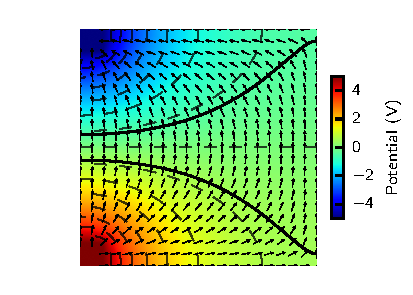
\includegraphics[width=7cm]{figures/classical-vdP.pdf}};

    \draw (-4,-4)--(-10,-4) to[current source, bipoles/length=1.5cm] (-10,4)--(-4,4);
    \node at(-10,0)[left=12pt]{$I_{34}$}; 

    \draw (4,-4)--(10,-4) to[rmeter, t = V, bipoles/length=1.5cm] (10,4)--(4,4);
    \node at(10,0)[right=12pt]{$V_{21}$}; 


    % Draw some TikZ elements
    \draw[thick, black] (-4,-4)--(4,-4)--(4,4)--(-4,4)--(-4,-4);
    \filldraw[fill = black!50, draw = black] (-5,-5)--(-3,-5)--(-3,-3)--(-5,-3)--(-5,-5);
    \filldraw[fill = black!50, draw = black] (5,-5)--(3,-5)--(3,-3)--(5,-3)--(5,-5);
    \filldraw[fill = black!50, draw = black] (-5,5)--(-3,5)--(-3,3)--(-5,3)--(-5,5);
    \filldraw[fill = black!50, draw = black] (5,5)--(3,5)--(3,3)--(5,3)--(5,5);
    \node[font=\large\bfseries] at (-4,-4) {4};
    \node[font=\large\bfseries] at (4,-4) {1};
    \node[font=\large\bfseries] at (-4,4) {3};
    \node[font=\large\bfseries] at (4,4) {2};
\end{circuitikz}